\section{Results}
\label{sec:results}

\subsection{Correct-message acceptance and erasures}

Figure~\ref{fig:acceptance} and Table~\ref{tab:cells} report every
confirmation cell. Under unit-average power, the equal-weight grid summary
is 784 correct acceptances in 1536 records (51.0\%); under unit-peak power,
it is 686/1536 (44.7\%). The profile totals are 414/768 and 370/768 for
moderate and hard fading at unit-average power, and 367/768 and 319/768 at
unit-peak power. These fractions summarize this deliberately balanced SNR
grid, rather than an operating distribution of HF conditions.

\begin{figure}[ht]
\centering
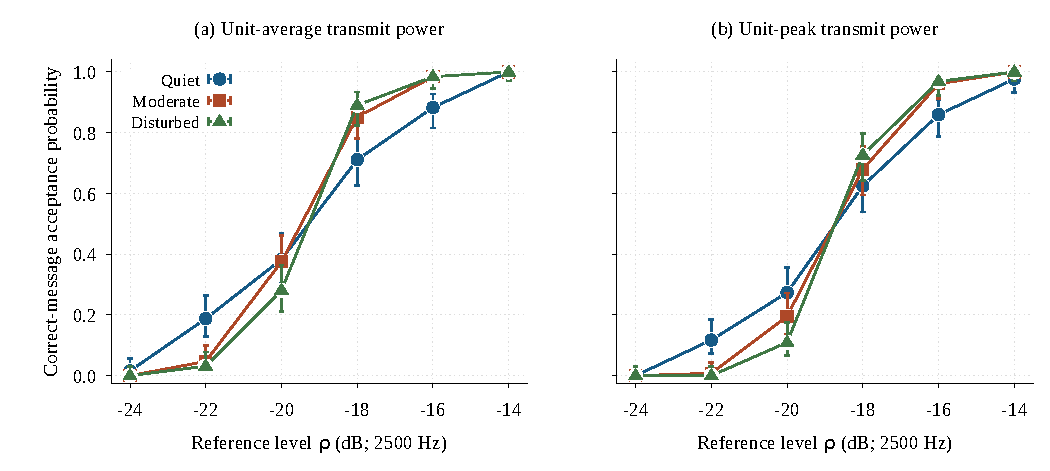
\includegraphics[width=\textwidth]{study/figures/acceptance.pdf}
\caption{Correct-message acceptance with pointwise 95\% Wilson intervals;
128 frames per point. Lines connect the measured points. The horizontal
axis is the unit-reference level $\rho$. In (a) it equals average transmit
SNR in 2500\,Hz; in (b) average transmit SNR is approximately 0.711\,dB lower.
The two panels reuse the same randomized cases.}
\label{fig:acceptance}
\end{figure}

\begin{table}[ht]
\centering\small
\begin{tabular}{@{}rll@{}}
\toprule
Reference $\rho$ & Moderate: $k/128$, rate [95\% CI] & Hard: $k/128$, rate [95\% CI] \\
\midrule
\multicolumn{3}{l}{\textit{Unit-average power}} \\
$-24$\,dB & 0/128, 0.000 [0.000, 0.029] & 0/128, 0.000 [0.000, 0.029] \\
$-22$\,dB & 2/128, 0.016 [0.004, 0.055] & 1/128, 0.008 [0.001, 0.043] \\
$-20$\,dB & 42/128, 0.328 [0.253, 0.413] & 17/128, 0.133 [0.085, 0.202] \\
$-18$\,dB & 115/128, 0.898 [0.834, 0.940] & 97/128, 0.758 [0.677, 0.824] \\
$-16$\,dB & 127/128, 0.992 [0.957, 0.999] & 127/128, 0.992 [0.957, 0.999] \\
$-14$\,dB & 128/128, 1.000 [0.971, 1.000] & 128/128, 1.000 [0.971, 1.000] \\
\midrule
\multicolumn{3}{l}{\textit{Unit-peak power}} \\
$-24$\,dB & 0/128, 0.000 [0.000, 0.029] & 0/128, 0.000 [0.000, 0.029] \\
$-22$\,dB & 0/128, 0.000 [0.000, 0.029] & 0/128, 0.000 [0.000, 0.029] \\
$-20$\,dB & 18/128, 0.141 [0.091, 0.211] & 8/128, 0.062 [0.032, 0.118] \\
$-18$\,dB & 95/128, 0.742 [0.660, 0.810] & 60/128, 0.469 [0.384, 0.555] \\
$-16$\,dB & 126/128, 0.984 [0.945, 0.996] & 123/128, 0.961 [0.912, 0.983] \\
$-14$\,dB & 128/128, 1.000 [0.971, 1.000] & 128/128, 1.000 [0.971, 1.000] \\
\bottomrule
\end{tabular}

\caption{Correct acceptances and pointwise 95\% Wilson intervals.
Every cell has zero incorrect acceptances; its erasure count is $128-k$.
Rates are dimensionless. Full erasure and incorrect-acceptance intervals
are supplied in \texttt{study/cells.csv}.}
\label{tab:cells}
\end{table}

At $-24\dB$, none of the four conditions accepts a correct message. At
$-14\dB$, every condition accepts all 128 messages; the Wilson interval
for each 128/128 cell is approximately $[0.971,1]$, so the observation does
not establish error-free operation. The transition between these limits
is resolved only at 2\,dB increments. No incorrect accepted message occurs
in any of the 3072 signal records; all remaining outcomes are erasures.
Because the power settings are paired, those records do not constitute
3072 independent opportunities for an undetected error.

\subsection{The 50\% acceptance crossing}

\begin{table}[ht]
\centering\small
\begin{tabular}{@{}llcc@{}}\toprule
Profile & Power setting & 50\% crossing & 95\% grid bracket \\
\midrule
Moderate & Average & $-19.4$\,dB & $[-20, -18]$\,dB \\
Hard & Average & $-18.8$\,dB & $[-20, -18]$\,dB \\
Moderate & Peak & $-18.8$\,dB & $[-20, -18]$\,dB \\
Hard & Peak & $-17.9$\,dB & $[-20, -16]$\,dB \\
\bottomrule\end{tabular}

\caption{Interpolated 50\% crossing in reference-level dB and conservative
95\% grid brackets under a monotone-response assumption. The bracket is
constructed from six simultaneous exact binomial intervals per curve.
Its width reflects sampling uncertainty and grid resolution.}
\label{tab:thresholds}
\end{table}

Table~\ref{tab:thresholds} places the unit-average crossings near $-19.4$
and $-18.8\dB$. Both lie between the measured $-20$ and $-18\dB$ points.
The moderate unit-peak crossing is also in that interval. For hard fading
at unit-peak power, 60/128 messages succeed at $-18\dB$, giving an
interpolated crossing near $-17.9\dB$ between $-18$ and $-16\dB$.
Its conservative uncertainty bracket spans $[-20,-16]\dB$ because the
$-18\dB$ cell does not locate the true success probability securely on
either side of 0.5. Sub-decibel interpolated values describe the chosen
interpolation and should not be read as sub-decibel measurement resolution.

\subsection{Noise-only acceptance}

\begin{table}[ht]
\centering
\begin{tabular}{@{}lrrrr@{}}
\toprule
Lot & Captures & Raw FEC accepts & Final accepts & Gate exceedances \\
\midrule
Calibration & 2048 & 0 & 0 & 21 \\
Independent check & 4096 & 0 & 0 & 44 \\
\bottomrule
\end{tabular}
\caption{Noise-only outcomes. Gate exceedance alone is not acceptance;
the receiver also requires raw decoder success.}
\label{tab:noise}
\end{table}

The independently seeded check has zero false accepts in 4096 captures,
giving the upper bound in \eqref{eq:falsebound}, or about 0.0731\% per
15-second capture. The reference scales have counts 683, 683, 683, 683,
682, and 682 in increasing $\rho$ order. The pooled bound does not supply
a separate 95\% upper limit of the same size at each scale. Both lots also
have zero raw FEC acceptances, so the evidence-only exceedances in
Table~\ref{tab:noise} must not be reported as false decoded messages.

\subsection{Waveform duration, bandwidth, and peak power}

The active waveform has exactly 116,800 samples at 12\,kHz, including both
filter tails, for a duration of 9.733333333\,s. The physical summary uses
1536 unique confirmation waveforms once each; duplicated records from the
two power settings do not enlarge the waveform sample. Mean $B_{99}$ is
1958.731\,Hz and the largest observed value is 1998.724\,Hz. Mean PAPR is
0.710905\,dB and the largest observed value is 0.710951\,dB. These extrema
belong to the sampled payloads, not to an exhaustive search of the codebook.
The nearly fixed envelope peak makes unit-peak active-frame average power
approximately 0.8490 and energy approximately 8.2636 in normalized
power-seconds, compared with 1 and 9.7333 under unit-average normalization.

\begin{figure}[ht]
\centering
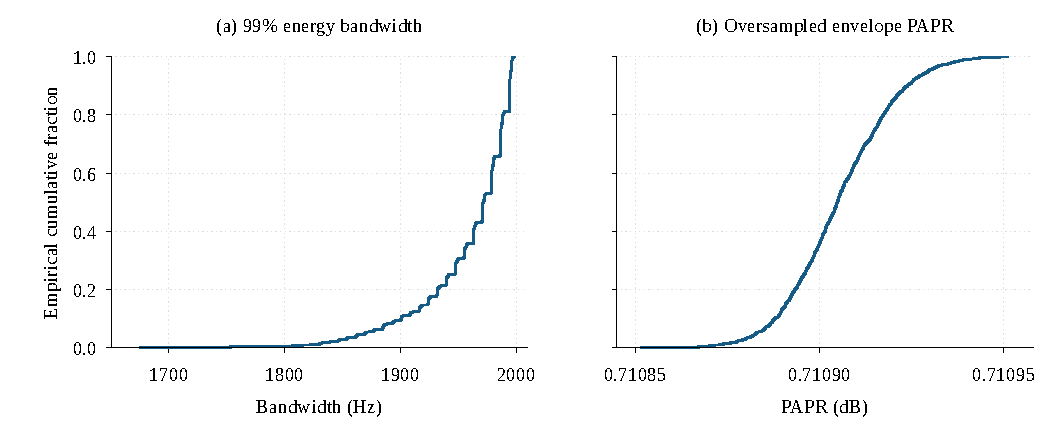
\includegraphics[width=\textwidth]{study/figures/physical.pdf}
\caption{Empirical cumulative distributions of the measured waveform
bandwidth and PAPR over 1536 unique confirmation cases. No channel fading
or noise enters these transmit-waveform measurements.}
\label{fig:physical}
\end{figure}
